% Sección de vida media del muón (práctica de muones)
% Requiere en el preámbulo:
%   \usepackage{graphicx}
%   \usepackage{subcaption}
% Ajustar la ruta "figuras/" según dónde estén los PDF.
% Figuras y números: muones/figuras/fig_decaimientos.py
% Referencias que cita (\cite{pdg}, \cite{suzuki}):
%   S. Navas et al. (Particle Data Group), Phys. Rev. D 110, 030001 (2024).
%   T. Suzuki, D. F. Measday y J. P. Roalsvig, Phys. Rev. C 35, 2212 (1987).

\section{Vida media del muón}

\subsection{Todos los decaimientos}

Con los módulos apilados (Fig.~\ref{fig:disp_apilados}) se registraron 978\,340
eventos. Un muón que frena dentro del detector y decae deja dos pulsos: el de
entrada y, más tarde, el del electrón del decaimiento. Se seleccionaron los
eventos que tienen un segundo pulso de al menos 60~mV en alguno de los tres
centelladores, entre 60 y 1400~ns después del de entrada. El límite inferior
asegura que el segundo pulso esté bien separado del primero y el superior lo fija
la ventana de adquisición, de 1{,}7~$\mu$s. Quedan 2542 decaimientos.

El tiempo entre los dos pulsos, $\Delta t$, se ajustó por máxima verosimilitud,
sin agrupar los datos en intervalos, con una exponencial normalizada en la ventana
$[a, b] = [60, 1400]$~ns,
\begin{equation}
    f(\Delta t;\tau) = \frac{e^{-\Delta t/\tau}}{\tau\left(e^{-a/\tau} - e^{-b/\tau}\right)} ,
    \label{eq:exponencial}
\end{equation}
cuyo único parámetro es la vida media $\tau$. El resultado es
\begin{equation}
    \tau = 1948^{+219}_{-179}~\text{ns} ,
\end{equation}
donde la incerteza es el intervalo en el que el logaritmo de la verosimilitud baja
$1/2$ respecto de su máximo. La Fig.~\ref{fig:decaimientos_todos} muestra que la
exponencial describe bien los datos ($\chi^2 = 17{,}6$ con 18 grados de libertad).

\begin{figure}[htbp]
    \centering
    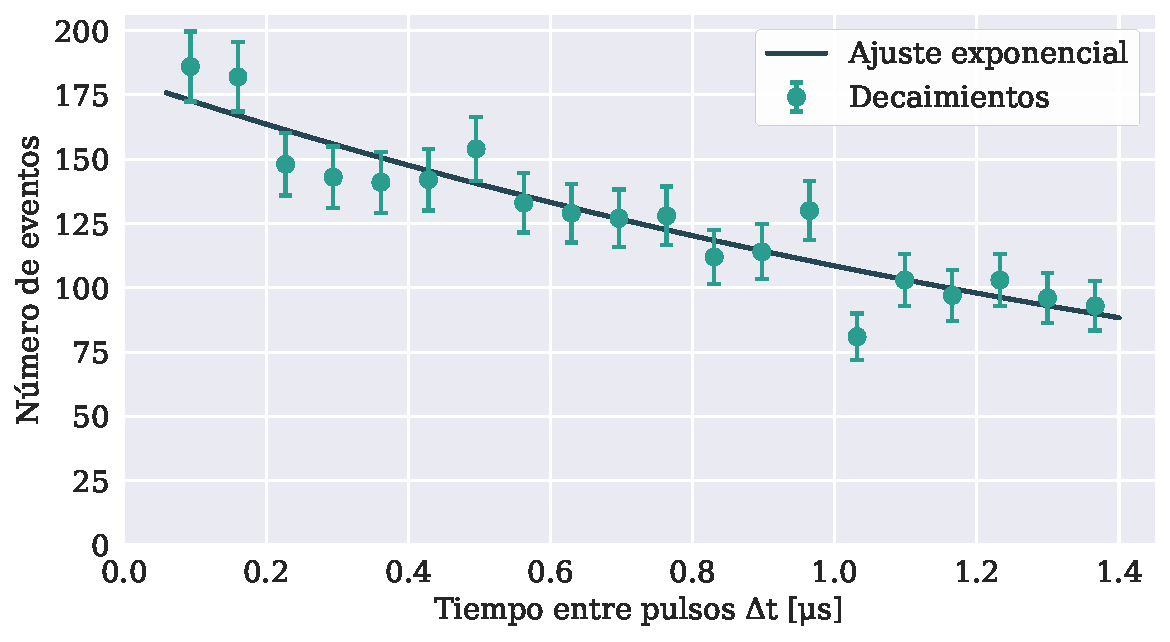
\includegraphics[width=0.85\textwidth]{figuras/decaimientos_todos.pdf}
    \caption{Distribución del tiempo entre el pulso de entrada del muón y el del
    electrón, $\Delta t$, para los 2542 decaimientos seleccionados. Cada punto es el
    número de eventos $N$ en un intervalo de 67~ns y las barras, $\sqrt{N}$. La curva
    es el ajuste de una exponencial (Ec.~\ref{eq:exponencial}) por máxima
    verosimilitud sobre los datos sin agrupar: $\tau = 1948^{+219}_{-179}$~ns
    ($\chi^2 = 17{,}6$ con 18 grados de libertad).}
    \label{fig:decaimientos_todos}
\end{figure}

El valor obtenido es menor que la vida media del muón libre,
$\tau_\mu = 2197$~ns~\cite{pdg}, aunque la diferencia, de 249~ns, es de apenas
1{,}1 veces la incerteza. Un valor más bajo es lo que se espera cuando los muones
decaen dentro de un material. Los muones positivos frenados decaen con la vida
media libre. Los negativos, en cambio, quedan ligados a un átomo del material y
pueden ser capturados por el núcleo ($\mu^- + p \to n + \nu_\mu$) antes de decaer.
La captura compite con el decaimiento, de modo que los $\mu^-$ desaparecen más
rápido,
\begin{equation}
    \frac{1}{\tau_{\mu^-}} = \frac{1}{\tau_\mu} + \Lambda_\text{cap} ,
\end{equation}
y los que llegan a decaer lo hacen con esa vida media más corta. La tasa de captura
$\Lambda_\text{cap}$ crece rápidamente con el número atómico: en el carbono del
plástico centellador $\tau_{\mu^-} = 2026$~ns, apenas menor que la libre, mientras
que en el hierro es de solo 206~ns~\cite{suzuki}. La muestra mezcla muones de las
dos cargas, frenados en el plástico y en la placa de hierro, y una única
exponencial ajustada a esa mezcla da una vida media efectiva menor que la del muón
libre.

\subsection{Decaimientos en el hierro y en el plástico}

Si esta explicación es correcta, la componente rápida debe aparecer solo en los
muones que frenan en el hierro. Para ponerlo a prueba se separaron los
decaimientos en dos grupos, según en qué centelladores hay pulso de entrada:
\begin{itemize}
    \item \textbf{Frena en el hierro} (1888 eventos): pulso de entrada en los
    centelladores 1 y 2, y no en el 3. El muón no llegó al centellador 3.
    \item \textbf{Frena en el centellador 3} (654 eventos): pulso de entrada en los
    tres centelladores. El muón cruzó el hierro y frenó en el plástico del
    centellador 3.
\end{itemize}

A cada grupo se le ajustó una exponencial (Ec.~\ref{eq:exponencial}) y la suma de
dos,
\begin{equation}
    g(\Delta t) = \phi\, f(\Delta t;\tau_\text{r}) + (1-\phi)\, f(\Delta t;\tau_\text{l}) ,
    \label{eq:dos_exponenciales}
\end{equation}
con una vida media rápida $\tau_\text{r}$, una lenta $\tau_\text{l}$ y la fracción
$\phi$ de eventos de la componente rápida, las tres libres. Los resultados están
en la Tabla~\ref{tab:dos_grupos} y en la Fig.~\ref{fig:dos_grupos}. La mejora del
ajuste al agregar la segunda exponencial se mide con el aumento del logaritmo de
la verosimilitud, $2\,\Delta\ln L$. Para saber si esa mejora es significativa, para
cada grupo se generaron 200 muestras simuladas con una sola exponencial y el mismo
número de eventos, y se las ajustó de la misma manera. La probabilidad $p$ de la
tabla es la fracción de esas muestras en las que la segunda exponencial mejora el
ajuste tanto o más que en los datos, es decir, la probabilidad de obtener esa
mejora por azar cuando no hay una segunda componente.

\begin{table}[htbp]
    \centering
    \begin{tabular}{lcc}
        \hline
         & Frena en el hierro & Frena en el centellador 3 \\
        \hline
        Eventos & 1888 & 654 \\
        \hline
        \multicolumn{3}{l}{\textit{Una exponencial}} \\
        $\tau$ [ns] & $1817^{+224}_{-179}$ & $2454^{+816}_{-491}$ \\
        $\chi^2$ / grados de libertad & $17{,}3$ / 18 & $14{,}6$ / 18 \\
        \hline
        \multicolumn{3}{l}{\textit{Dos exponenciales}} \\
        $\tau_\text{r}$ [ns] & 42 (menor que 105) & 203 (sin determinar) \\
        $\tau_\text{l}$ [ns] & $2025^{+252}_{-236}$ & 2875 (mayor que 2101) \\
        $\phi$ [\%] & $1{,}5^{+1{,}5}_{-0{,}7}$ & $2{,}2$ (menor que $37{,}5$) \\
        $\chi^2$ / grados de libertad & $15{,}0$ / 16 & $14{,}3$ / 16 \\
        \hline
        \multicolumn{3}{l}{\textit{Mejora al agregar la segunda exponencial}} \\
        $2\,\Delta\ln L$ & $3{,}20$ & $0{,}18$ \\
        Probabilidad de obtenerla por azar, $p$ & 7~\% & 53~\% \\
        \hline
    \end{tabular}
    \caption{Ajustes de una y de dos exponenciales al tiempo entre pulsos de cada
    grupo, en la ventana de 60 a 1400~ns. Las incertezas y las cotas son intervalos
    de 68~\%. El $\chi^2$ se calculó sobre los histogramas de la
    Fig.~\ref{fig:dos_grupos}.}
    \label{tab:dos_grupos}
\end{table}

\begin{figure}[htbp]
    \centering
    \begin{subfigure}[b]{0.8\textwidth}
        \centering
        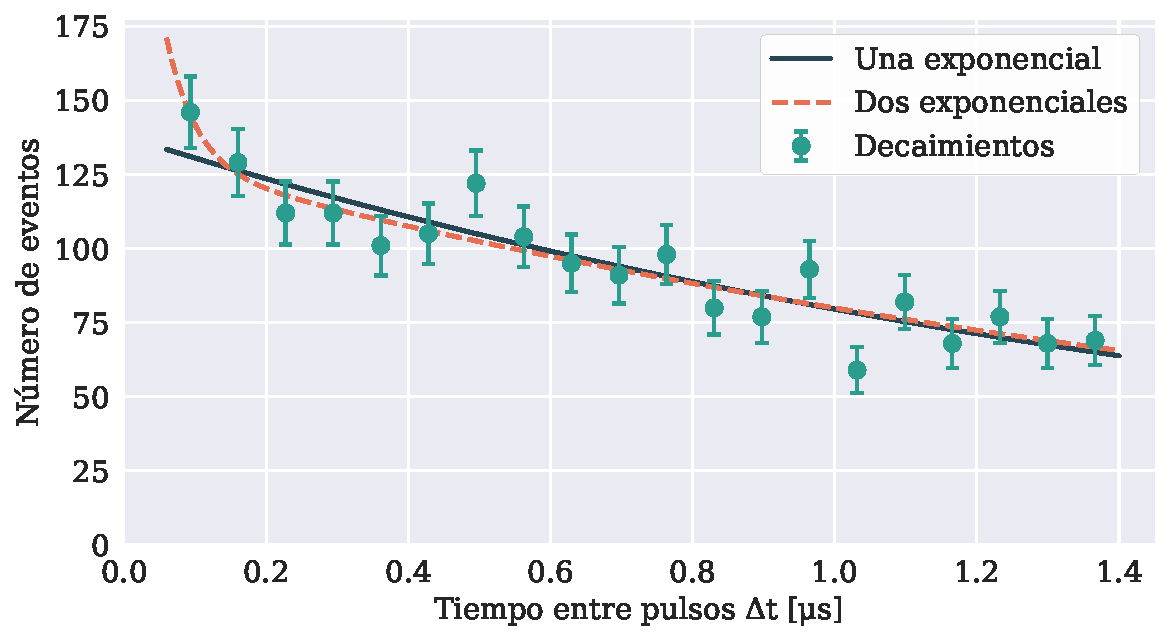
\includegraphics[width=\linewidth]{figuras/decaimientos_hierro.pdf}
        \caption{Frena en el hierro.}
        \label{fig:decaimientos_hierro}
    \end{subfigure}

    \vspace{0.5em}
    \begin{subfigure}[b]{0.8\textwidth}
        \centering
        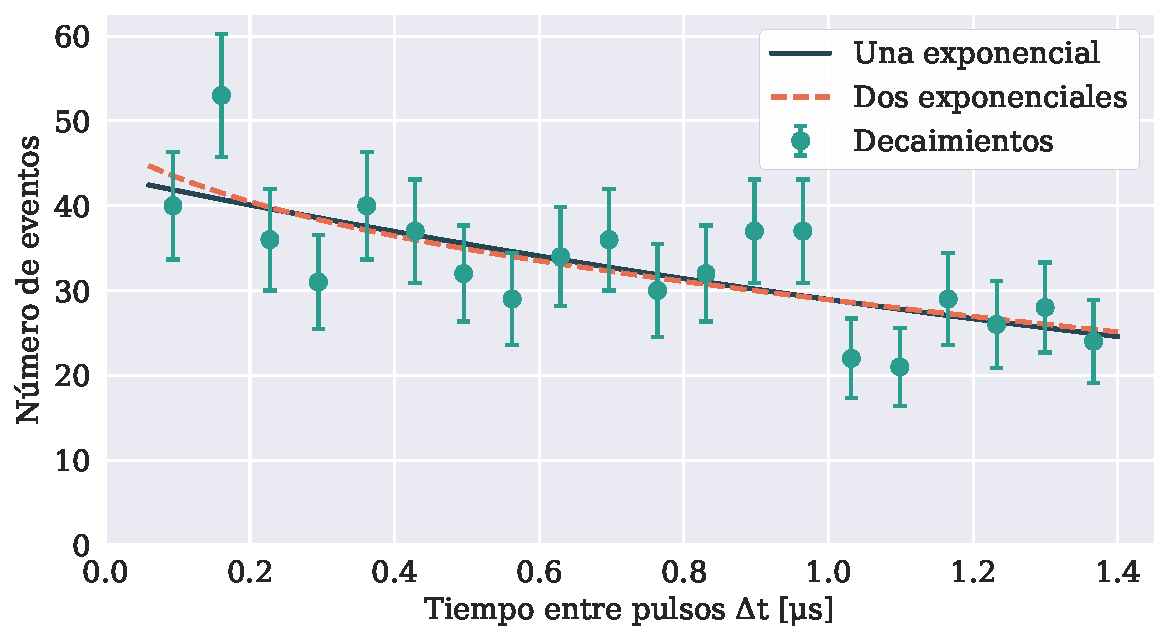
\includegraphics[width=\linewidth]{figuras/decaimientos_centellador3.pdf}
        \caption{Frena en el centellador 3.}
        \label{fig:decaimientos_centellador3}
    \end{subfigure}

    \caption{Distribución del tiempo entre pulsos $\Delta t$ para (a)~los 1888
    muones que frenan en el hierro y (b)~los 654 que lo cruzan y frenan en el
    centellador 3. Cada punto es el número de eventos $N$ en un intervalo de 67~ns
    y las barras, $\sqrt{N}$. Las curvas son los ajustes de una exponencial
    (Ec.~\ref{eq:exponencial}, línea llena) y de la suma de dos
    (Ec.~\ref{eq:dos_exponenciales}, línea de trazos), con los parámetros de la
    Tabla~\ref{tab:dos_grupos}. En (a) la segunda exponencial describe el exceso de
    eventos a $\Delta t$ cortos; en (b) las dos curvas casi coinciden.}
    \label{fig:dos_grupos}
\end{figure}

Con una sola exponencial, la vida media de los muones que frenan en el hierro,
$1817^{+224}_{-179}$~ns, es menor que la libre, mientras que la de los que frenan
en el centellador 3, $2454^{+816}_{-491}$~ns, es compatible con ella y con la
esperada en el plástico.

Al agregar la segunda exponencial, los dos grupos se comportan distinto. En el
grupo del hierro el ajuste mejora ($2\,\Delta\ln L = 3{,}20$): la componente rápida
describe un exceso de eventos a $\Delta t$ cortos
(Fig.~\ref{fig:decaimientos_hierro}) y la lenta,
$\tau_\text{l} = 2025^{+252}_{-236}$~ns, queda compatible con la vida media del
muón libre. Una mejora así aparece por azar en el 7~\% de las muestras simuladas.
Los datos no alcanzan para medir la vida media rápida: el ajuste da 42~ns, pero si
se fijan las dos vidas medias en los valores esperados, 206 y 2197~ns, la
verosimilitud apenas empeora ($\Delta\ln L = 0{,}86$) y la fracción rápida resulta
de 3{,}7~\%. En el grupo del centellador 3, en cambio, la segunda exponencial no
mejora el ajuste ($2\,\Delta\ln L = 0{,}18$, que se obtiene por azar en el 53~\% de
los casos), sus parámetros quedan sin determinar y la fracción rápida es compatible
con cero.

En resumen, la componente rápida aparece en los muones que frenan en el hierro y
no en los que frenan en el plástico. Esto es consistente con que la vida media
medida con todos los eventos resulte menor que la del muón libre por la captura de
los $\mu^-$ en el hierro. La evidencia es débil: una probabilidad de 7~\% no
alcanza el 5~\% que se usa habitualmente para considerar significativa una mejora,
de modo que los datos no permiten afirmarlo. La limitación principal es la ventana
de adquisición, más corta que una vida media.
